\clearpage
\section{Vestments, Ministries, and Communion Vessels}
\PCDPlateHeader{Plate VIII --- Ordained Vesture at Mass}{Standing figures to common scale; insets not to scale}
\ifdefined\TriptychPrintEdition
\begin{center}
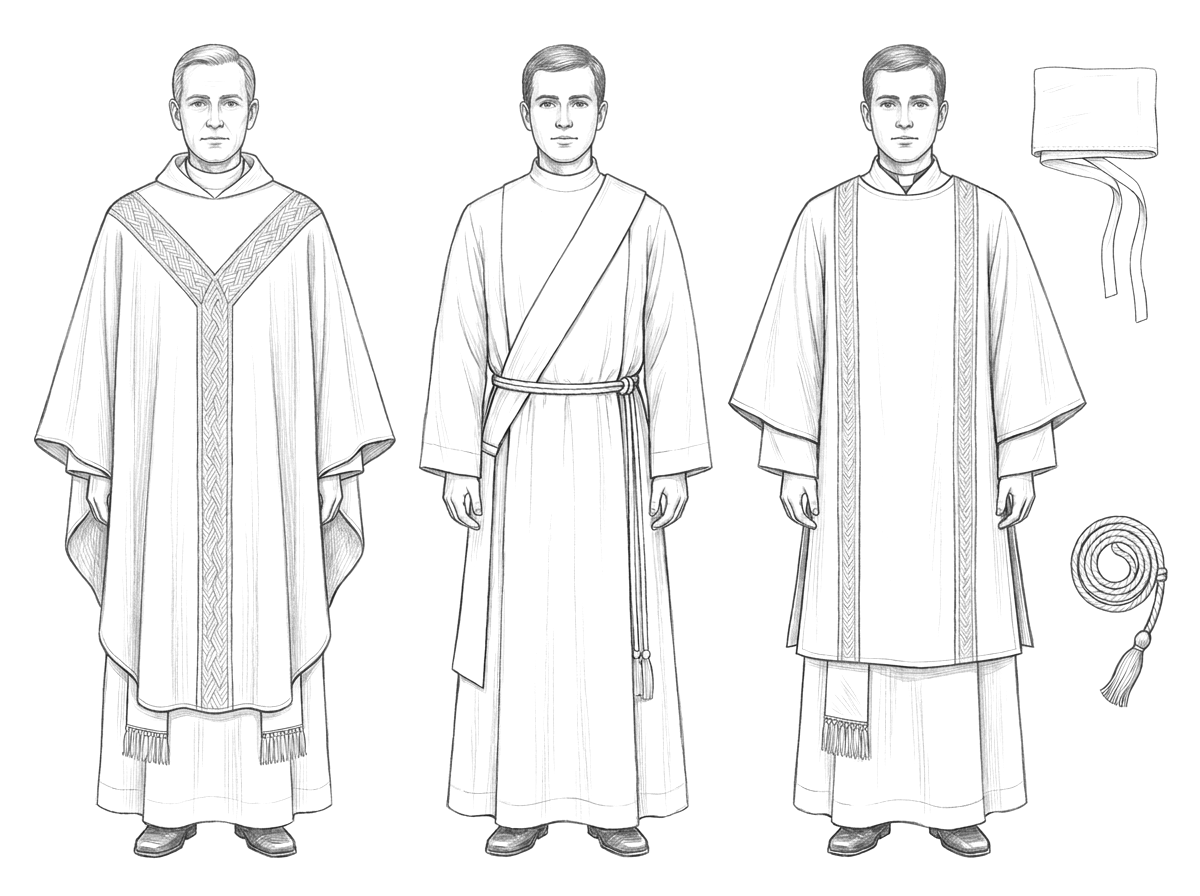
\includegraphics[width=0.92\linewidth,height=3.55in,keepaspectratio]{liturgy/roman-rite/postconciliar/2008-latin-2011-us-english/reference/roman-sanctuary-dictionary/shared/artwork/graphite/pc-art-08-priest-deacon-vesture.png}
\end{center}
\PCDPositionKey{Left: Priest in Alb, Amice, straight vertical Stole, and Y-orphrey Chasuble; center: Deacon in Alb, Cincture, and diagonal Stole from left shoulder to right hip without dalmatic; right: Deacon in Alb and sleeved Dalmatic worn over the diagonal Stole (fringed tip peeking at deacon's right side); far right insets: folded Amice with ties (top) and coiled tasseled Cincture (bottom).}
\else
\textbf{Visual Plate Summary (Plate VIII --- Ordained Vesture at Mass, Standing figures to common scale; insets not to scale):} Worn monochrome graphite vestment study comparing priest and deacon at common scale: left, a priest vested in ankle-length white alb, amice at collar, straight vertical stole ends visible below a flowing Gothic chasuble with Y-shaped orphrey; center, a deacon in white alb and tied cord cincture wearing his stole diagonally from left shoulder across the chest to his right hip; right, a deacon vested in a wide-sleeved dalmatic with vertical clavi stripes worn over the diagonal stole, whose fringed end peeks below the deacon's right hem; far right margin insets show a folded rectangular amice with cloth ties above and a coiled tasseled cincture below.

\textbf{Reading order and object placement:} Left: Priest in Alb, Amice, straight vertical Stole, and Y-orphrey Chasuble; center: Deacon in Alb, Cincture, and diagonal Stole from left shoulder to right hip without dalmatic; right: Deacon in Alb and sleeved Dalmatic worn over the diagonal Stole (fringed tip peeking at deacon's right side); far right insets: folded Amice with ties (top) and coiled tasseled Cincture (bottom).
\fi

\label{pc-obj-alb}
\PCDEntryHead{Alb}{Alba}{required}{N31}
\PCDField{Also called}{White Tunic; \textit{Tunica alba}}
Beneath the colorful outer vestments of priest and deacon, every ordained and instituted minister in the sanctuary wears the same ankle-length white alb (GIRM 336). In the United States, altar servers and lay readers often wear the alb as well (US GIRM 339), visually uniting everyone who ministers around the altar in the white garment of Christian Baptism.

\PCDField{On the plate}{Worn beneath chasuble, diagonal stole, and dalmatic across all three figures (Plate VIII), and under cope and humeral veil (Plate IX)}
\PCDField{Symbolism}{As the single white garment shared by ordained and instituted ministers of every rank, the alb outwardly recalls baptismal dignity in Christ (GIRM 335--336), echoing St. Paul, ``For as many of you as have been baptized in Christ have put on Christ'' (Gal 3:27), and the saints who ``have washed their robes and have made them white in the blood of the Lamb'' (Apoc 7:14). Outside the norms of the General Instruction, the traditional Roman sacristy vesting prayer asks the Lord to make the minister pure and white in the blood of the Lamb, and Amalarius of Metz interprets the loose linen tunic as Christian freedom and bodily discipline. (GIRM 335--336; Gal 3:27; Apoc 7:13--14; traditional Roman sacristy vesting prayer (Ad Albam); Amalarius of Metz, Liber Officialis II.18)}
\PCDField{Relation to the 1962 Missal}{\PCDTag{changed use} In the 1962 Roman Missal, the alb was worn solely by ordained sacred ministers at Mass (bishop, priest, deacon, and subdeacon, RS I.2--3), while altar servers and minor clerics wore cassock and surplice (RS II.1, VI.8). Under the 2002/2008 GIRM, the alb becomes the universal common garment of all ordained and instituted ministers, may never be replaced by a surplice under a chasuble, dalmatic, or stole alone (GIRM 336), and in the United States is also permitted for altar servers, readers, and other lay ministers (US GIRM 339).}
\PCDEntryRule

\label{pc-obj-cincture}
\PCDEntryHead{Cincture}{Cingulum}{required}{N32}
\PCDField{Also called}{Girdle; Waist Cord; \textit{Zona}}
Because a traditional linen alb is cut generously, a woven rope cincture gathers it comfortably at the waist and adjusts the hem so it clears the floor cleanly. Under current Roman law, the cincture is required whenever an alb is not tailored to fit smoothly on its own (GIRM 336).

\PCDField{On the plate}{Tied at waist of center deacon and coiled in lower right inset (Plate VIII)}
\PCDField{Symbolism}{The General Instruction prescribes the cincture strictly for the practical task of fastening an unfitted alb at the waist (GIRM 336). Distinct from that rubrical rule, the traditional Roman sacristy vesting prayer asks God to gird the minister with the belt of purity, continence, and chastity, echoing the Gospel and Epistles---``Let your loins be girt and lamps burning in your hands'' (Luke 12:35) and ``Stand therefore, having your loins girt about with truth'' (Eph 6:14)---while Amalarius of Metz likewise reads the cincture as an emblem of self-mastery. (Practical norm: GIRM 336; devotional tradition: Roman sacristy vesting prayer (Ad Cingulum); Luke 12:35; Eph 6:14; Amalarius of Metz, Liber Officialis II.22)}
\PCDField{Relation to the 1962 Missal}{\PCDTag{optional} In the 1962 Roman Missal, the cincture was unconditionally mandatory with every alb both to gather the tunic and to anchor the priest's crossed stole across the breast (RS I.3). Under the 2002/2008 GIRM, the cincture becomes conditionally optional whenever an alb is tailored to fit cleanly without one (GIRM 336), and the priest's stole hangs straight rather than crossing through the cincture (GIRM 340).}
\PCDEntryRule

\label{pc-obj-amice}
\PCDEntryHead{Amice}{Amictus}{required}{N33}
\PCDField{Also called}{Shoulder Cloth}
Often noticed only as a crisp white linen fold framing the priest's collar beneath the chasuble, the amice is a practical shoulder cloth fastened with long waist ties. Current Roman law calls for it whenever an alb's neckline does not completely cover ordinary clothing at the neck (GIRM 336).

\PCDField{On the plate}{At collar of priest on left and folded with tie strings in upper right inset (Plate VIII)}
\PCDField{Symbolism}{The General Instruction assigns the amice a practical purpose---covering ordinary attire at the neck whenever the alb leaves it exposed (GIRM 336). Distinct from that practical rule, the traditional Roman sacristy vesting prayer---recalling the custom of resting the amice momentarily on the head before lowering it to the shoulders---prays for the helmet of salvation against demonic assaults, echoing St. Paul: ``And take unto you the helmet of salvation and the sword of the Spirit (which is the word of God)'' (Eph 6:17). Amalarius of Metz reads the cloth encircling the neck as a guard over speech, citing the Psalms, ``I have set a guard to my mouth'' (Ps 38:2 [Heb 39:1]) and ``Set a watch, O Lord, before my mouth'' (Ps 140:3 [Heb 141:3]). (Practical norm: GIRM 336; devotional tradition: Roman sacristy vesting prayer (Ad Amictum); Eph 6:17; Ps 38:2 [Heb 39:1]; Ps 140:3 [Heb 141:3]; Amalarius of Metz, Liber Officialis II.17)}
\PCDField{Relation to the 1962 Missal}{\PCDTag{optional} In the 1962 Roman Missal, the amice was unconditionally required as the first Mass vestment for every bishop, priest, deacon, and subdeacon, kissed at its center cross and placed briefly upon the head before settling on the shoulders (RS I.3). Under the 2002/2008 GIRM, the amice is conditionally required only when the alb fails to cover ordinary attire at the neck (GIRM 336).}
\PCDEntryRule

\label{pc-obj-stole}
\PCDEntryHead{Stole}{Stola}{required}{N34}
\PCDField{Also called}{Priestly Stole; Diaconal Stole}
More than any other garment, the woven stole identifies an ordained minister at a glance. In the postconciliar Roman Rite, both bishop and priest wear it hanging straight down in front of the chest, while the deacon wears it sash-like from his left shoulder to his right hip under the dalmatic (GIRM 340).

\PCDField{On the plate}{Hanging straight below priest's chasuble at left; worn diagonally from left shoulder to right hip on center deacon and beneath right deacon's dalmatic with tip peeking at his right hem (Plate VIII)}
\PCDField{Symbolism}{The stole outwardly signifies ordained ministry within the Body of Christ, distinguishing episcopal and presbyteral order from diaconal order by the manner in which it is worn (GIRM 335, 340). In devotional tradition distinct from the General Instruction, the traditional Roman sacristy vesting prayer asks the Lord to restore the robe of immortality lost by our first parents, while Amalarius of Metz sees in the stole the sweet yoke of the Gospel (Matt 11:29--30). (GIRM 335, 340; traditional Roman sacristy vesting prayer (Ad Stolam); Matt 11:29--30; Amalarius of Metz, Liber Officialis II.20)}
\PCDField{Relation to the 1962 Missal}{\PCDTag{changed use} While the deacon's diagonal wearing from left shoulder to right hip continues unchanged from 1962, the 1962 Roman Missal required a priest celebrating Mass to cross the stole across his breast and anchor it with the cincture, reserving straight hanging to bishops and prelates (RS I.3--4). Under GIRM 340, every priest now wears the stole hanging straight down in front of his chest.}
\PCDEntryRule

\label{pc-obj-chasuble}
\PCDEntryHead{Chasuble}{Casula}{required}{N35}
\PCDField{Also called}{Mass Vestment; \textit{Planeta}}
Enveloping the priest from shoulders to shins, the chasuble is the unmistakable outer garment of the Eucharistic celebrant at Mass (GIRM 337). Its seasonal color---white for Easter and Christmas, red for Pentecost and martyrs, green for Ordinary Time, violet for Advent and Lent, rose twice a year, and black, white, or gold where appointed---sets the visual tone of the day's celebration (GIRM 346).

\PCDField{On the plate}{Left figure, Y-orphrey outer vestment of priest celebrant (Plate VIII)}
\PCDField{Symbolism}{The chasuble is the outer liturgical sign proper to the priest celebrant's presidential and sacrificial office at Mass (GIRM 335, 337). In devotional tradition distinct from the General Instruction, the traditional Roman sacristy vesting prayer echoes Christ's words, ``For my yoke is sweet and my burden light'' (Matt 11:30), Christian tradition connects its all-enveloping mantle with charity---``But above all these things have charity, which is the bond of perfection'' (Col 3:14)---and Amalarius of Metz sees in it the works of justice and holiness. (GIRM 335, 337; Matt 11:30; Col 3:14; traditional Roman sacristy vesting prayer (Ad Casulam); Amalarius of Metz, Liber Officialis II.19)}
\PCDField{Relation to the 1962 Missal}{\PCDTag{continued} Both the 1962 Roman Missal (RG 133--134; RS I.4) and the 2002/2008 GIRM (119a, 337) prescribe the chasuble as the proper Mass vestment of the priest celebrant over alb and stole. Postconciliar rubrics additionally allow the chasuble for rites immediately joined to Mass such as the Sunday sprinkling, Ash Wednesday ashes, and funeral commendation (Tres abhinc annos 26; GIRM 337), emphasize graceful form and noble fabric over heavy ornament (GIRM 344), and introduce a narrow omission faculty for non-principal concelebrants in genuine need (GIRM 209; RS 124).}
\PCDEntryRule

\label{pc-obj-dalmatic}
\PCDEntryHead{Dalmatic}{Dalmatica}{provided}{N36}
\PCDField{Also called}{Deacon's Dalmatic; \textit{Dalmatica diaconalis}}
Distinguished from the priest's flowing chasuble by its wide sleeves and twin vertical bands, the dalmatic has been the hallmark garment of the Roman deacon since late antiquity. Worn over the alb and the deacon's diagonal stole, it visually identifies the ordained minister who proclaims the Gospel, prepares the altar, and assists with the chalice.

\PCDField{On the plate}{Right figure, wide-sleeved rectangular outer vestment worn over the diagonal stole (Plate VIII)}
\PCDField{Symbolism}{The dalmatic outwardly manifests the diaconal order of service within the Body of Christ (GIRM 335, 338), and when worn by a bishop beneath his chasuble on solemnities it expresses the fullness of Holy Orders (CE 1984 no. 56). In devotional tradition distinct from the General Instruction, the traditional vesting prayer echoes Is 61:10 (``for he hath clothed me with the garments of salvation: and with the robe of justice he hath covered me''), while Amalarius of Metz links its wide sleeves to generous charity toward widows and orphans (James 1:27). (GIRM 335, 338; Caeremoniale Episcoporum (1984) 56; Is 61:10; James 1:27; traditional Roman vesting prayer; Amalarius of Metz, Liber Officialis II.21)}
\PCDField{Relation to the 1962 Missal}{\PCDTag{continued} The dalmatic continues from the 1962 Roman Missal (RG 137) as the proper outer vestment of the deacon over alb and diagonal stole. Postconciliar GIRM 338 introduces a limited omission faculty for necessity or lesser solemnity (discouraged by RS 125), while Caeremoniale Episcoporum (1984) no. 56 simplifies episcopal solemn vesting to a single dalmatic beneath the chasuble without a separate tunicle.}
\PCDEntryRule

\clearpage
\PCDPlateHeader{Plate IX --- Choir Dress and Solemn Ceremonial Vesture}{Standing figures to common scale}
\ifdefined\TriptychPrintEdition
\begin{center}
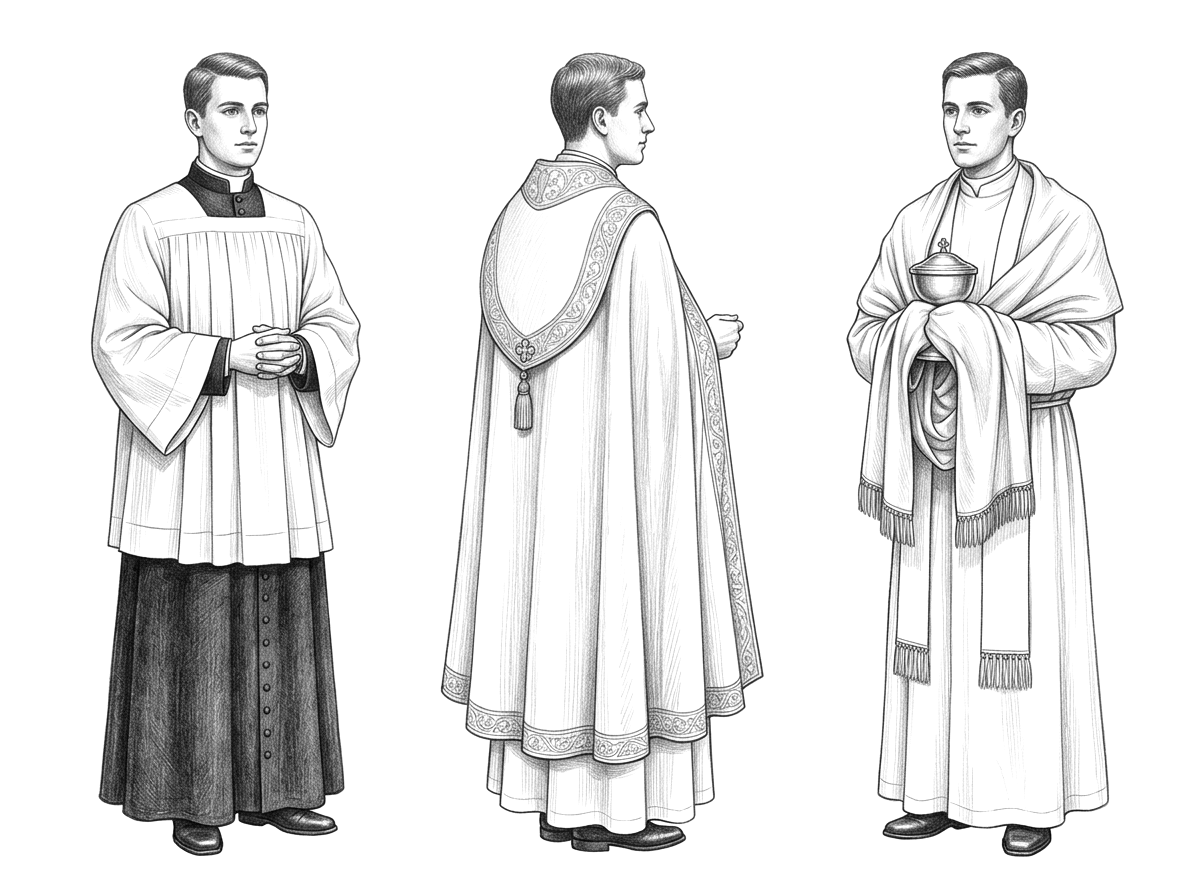
\includegraphics[width=0.92\linewidth,height=3.55in,keepaspectratio]{liturgy/roman-rite/postconciliar/2008-latin-2011-us-english/reference/roman-sanctuary-dictionary/shared/artwork/graphite/pc-art-09-black-cassock-surplice-cope.png}
\end{center}
\PCDPositionKey{Left: choir dress (deep black buttoned clerical Cassock beneath crisp white pleated Surplice); center: three-quarter rear view of semicircular Cope with ornamental hood shield and tassel over an Alb; right: Priest in Alb and straight Stole wearing a fringed Humeral Veil whose cloth completely envelops both hands supporting a closed lidded ciborium.}
\else
\textbf{Visual Plate Summary (Plate IX --- Choir Dress and Solemn Ceremonial Vesture, Standing figures to common scale):} Three-figure monochrome graphite garment study demonstrating high-contrast shading: left, a standing figure in clerical choir dress wearing a deep charcoal-black ankle-length buttoned cassock under a bright white pleated wide-sleeved surplice; center, three-quarter rear view of a flowing semicircular cope with embroidered hood shield and tassel worn over a white alb; right, three-quarter front view of a priest in alb and straight vertical stole draped in an oblong fringed humeral veil whose ends wrap completely over both hands as he holds a closed lidded ciborium.

\textbf{Reading order and object placement:} Left: choir dress (deep black buttoned clerical Cassock beneath crisp white pleated Surplice); center: three-quarter rear view of semicircular Cope with ornamental hood shield and tassel over an Alb; right: Priest in Alb and straight Stole wearing a fringed Humeral Veil whose cloth completely envelops both hands supporting a closed lidded ciborium.
\fi

\label{pc-obj-cassock-surplice}
\PCDEntryHead{Cassock and Surplice}{Vestis talaris et superpelliceum}{permitted}{N37}
\PCDField{Also called}{Choir Dress; Server's Cassock and Surplice; \textit{Talaris}; \textit{Superpelliceum}; \textit{Cotta}}
The stark contrast of a bright pleated white surplice over a black ankle-length cassock has clothed altar servers and choir clergy for centuries. While the postconciliar Roman Missal made the full-length white alb the common garment of ordained and instituted ministers at Mass, cassock and surplice continue as choir dress for non-concelebrating priests and as lawful, traditional attire for altar servers.

\PCDField{On the plate}{Left figure, deep charcoal-black ankle-length buttoned cassock under bright pleated white surplice (Plate IX)}
\PCDField{Relation to the 1962 Missal}{\PCDTag{changed use} In the 1962 Roman Missal, cassock and surplice were the standard vesture of altar servers, choir clergy, and priests administering many non-Mass rites with a stole (RS II.1, VI.8). Postconciliar GIRM 336 replaces surplice-and-stole with alb-and-stole whenever rubrics prescribe a stole alone or beneath chasuble/dalmatic, while retaining cassock and surplice for choir dress (RS 128) and permitting them for altar servers alongside the alb (US GIRM 339; CE 1984 no. 65).}
\PCDEntryRule

\label{pc-obj-cope}
\PCDEntryHead{Cope}{Pluviale}{provided}{N38}
\PCDField{Also called}{Processional Mantle; \textit{Cappa}}
Descending from the ancient hooded outdoor cloak (Latin pluviale, ``rain cloak''), the semicircular cope lends solemn beauty to Catholic processions, Solemn Vespers, and Eucharistic Benediction. Open in front and fastened at the chest by a clasp, it distinguishes non-Mass liturgical rites from the Eucharistic sacrifice, for which the priest vests in the chasuble.

\PCDField{On the plate}{Center figure, three-quarter rear view showing full semicircular cloak, embroidered hood shield, and tassel over an alb (Plate IX)}
\PCDField{Relation to the 1962 Missal}{\PCDTag{continued} The cope continues from 1962 usage in processions, solemn Office, and Eucharistic Benediction (GIRM 341; HCWEOM nn. 91--92). Following Tres abhinc annos (1967) no. 26 and GIRM 51 and 337, postconciliar rubrics permit the chasuble rather than requiring a cope for rites integrated directly into Mass such as the Sunday sprinkling rite and Ash Wednesday imposition of ashes.}
\PCDEntryRule

\label{pc-obj-humeral-veil}
\PCDEntryHead{Humeral Veil}{Velum humerale}{provided}{N39}
\PCDField{Also called}{Benediction Veil; \textit{Velum}}
During Eucharistic Benediction and solemn processions of the Blessed Sacrament, the priest or deacon drapes a long white fringed shawl---the humeral veil---across his shoulders and wraps its ends completely around his hands before lifting the monstrance or ciborium. By veiling the minister's hands, the liturgy makes visually unmistakable that it is Christ Himself, truly present in the Eucharist, who blesses His people.

\PCDField{On the plate}{Right figure, oblong fringed white cloth draped over shoulders with ends wrapping completely over both hands around a lidded ciborium (Plate IX)}
\PCDField{Symbolism}{Covering the minister's hands in clean white cloth while raising the monstrance or ciborium expresses profound reverence before Christ's Real Presence and visibly manifests that Christ Himself---not the human minister---imparts the Eucharistic blessing. (Holy Communion and Worship of the Eucharist Outside Mass (1973) nn. 91--92; Roman Missal (2008/2011), Evening Mass of the Lord's Supper)}
\PCDField{Relation to the 1962 Missal}{\PCDTag{changed use} In the 1962 Roman Missal, the humeral veil served both Eucharistic Benediction and processions and---at Solemn High Mass---the subdeacon, who wore it from Offertory to the Pater Noster to hold the empty paten (RS VII.9, X.8). After Paul VI's Ministeria quaedam (1972) suppressed the subdiaconate and the 1969/1970 Order of Mass omitted subdiaconal paten-holding, the humeral veil's liturgical use is dedicated exclusively to Eucharistic Benediction, processions, and Holy Thursday transfer.}
\PCDEntryRule

\clearpage
\PCDPlateHeader{Plate X --- Communion Under Both Kinds and Sacramental Vessels}{Not to common scale}
\ifdefined\TriptychPrintEdition
\begin{center}
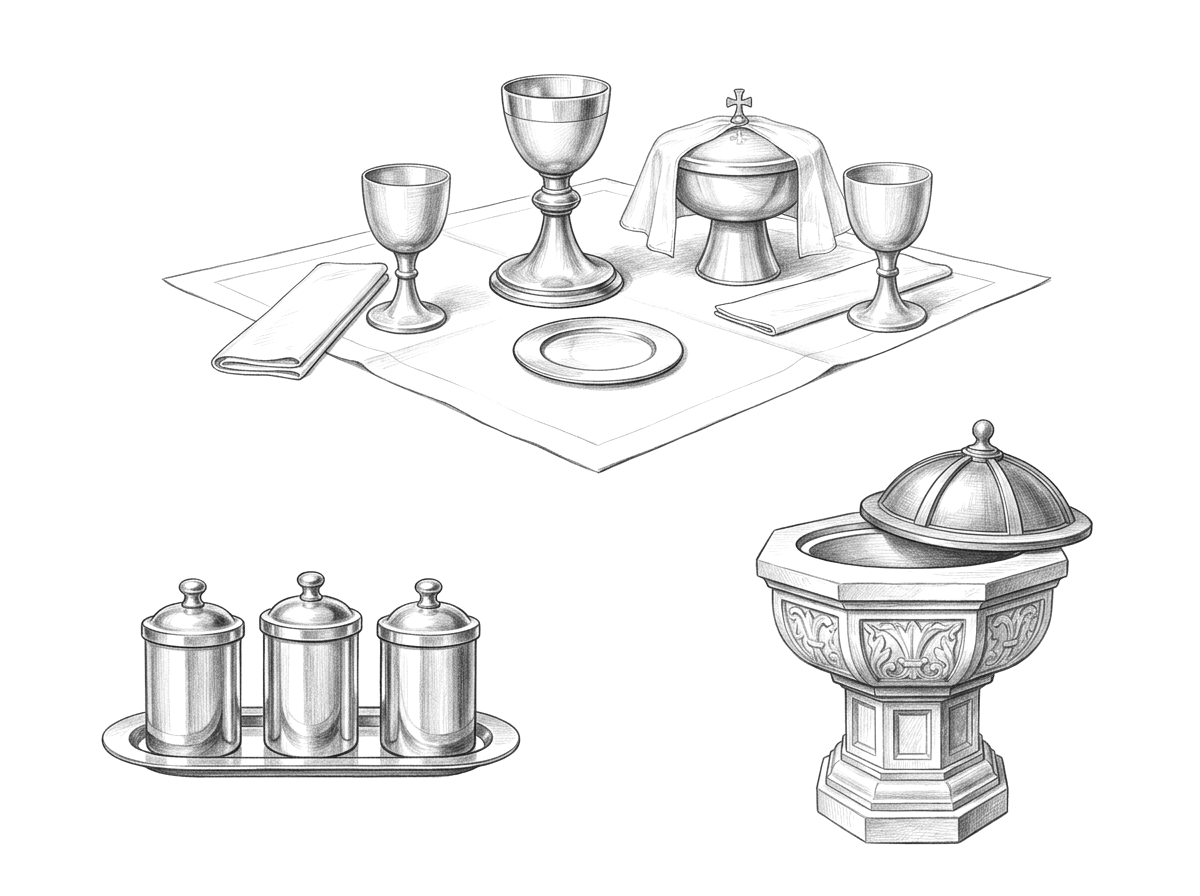
\includegraphics[width=0.92\linewidth,height=3.55in,keepaspectratio]{liturgy/roman-rite/postconciliar/2008-latin-2011-us-english/reference/roman-sanctuary-dictionary/shared/artwork/graphite/pc-art-10-communion-triduum-vessels.png}
\end{center}
\PCDPositionKey{Top: Communion under both kinds arrangement on an unfolded Corporal (principal Chalice, Paten, veiled covered Ciborium, and two footed Communion Cups each with a folded Purificator); bottom left: three cylindrical lidded metal Holy Oils Stocks on a tray (Sacred Chrism, Oil of Catechumens, Oil of the Sick); bottom right: carved octagonal stone Baptismal Font with removable domed cover ajar.}
\else
\textbf{Visual Plate Summary (Plate X --- Communion Under Both Kinds and Sacramental Vessels, Not to common scale):} Three-group monochrome graphite sacramental plate: top, an unfolded square corporal holding a central principal chalice, shallow paten, closed ciborium draped in a white veil, and two footed Communion cups each beside a folded purificator; bottom left, three matching cylindrical lidded metal holy-oil vessels resting on an oval metal tray without baked inscriptions; bottom right, an octagonal carved stone baptismal font on a pedestal with its domed cover resting slightly open to reveal the water basin rim.

\textbf{Reading order and object placement:} Top: Communion under both kinds arrangement on an unfolded Corporal (principal Chalice, Paten, veiled covered Ciborium, and two footed Communion Cups each with a folded Purificator); bottom left: three cylindrical lidded metal Holy Oils Stocks on a tray (Sacred Chrism, Oil of Catechumens, Oil of the Sick); bottom right: carved octagonal stone Baptismal Font with removable domed cover ajar.
\fi

\label{pc-obj-holy-oils-stocks}
\PCDEntryHead{Holy Oils and Oil Stocks}{Olea sancta et vasa oleorum}{required}{N40}
\PCDField{Also called}{Sacred Chrism (SC), Oil of Catechumens (OC), and Oil of the Sick (OI); oil stocks; chrismatory; oil urns; ambry (oil cabinet); \textit{Sanctum Chrisma}; \textit{Oleum catechumenorum}; \textit{Oleum infirmorum}; \textit{ampullae oleorum}; \textit{thecae}; \textit{armarium oleorum}}
Every year during Holy Week, the diocesan bishop gathers with his priests at the Chrism Mass to bless the Oil of the Sick and the Oil of Catechumens and to consecrate perfumed Sacred Chrism, sending fresh oils home to every parish. Kept in three matching lidded stocks inside a locked parish cabinet called an ambry, these oils trace the arc of a Catholic life: strengthening catechumens before Baptism, sealing the baptized and confirmed with the gift of the Holy Spirit, healing and fortifying the gravely ill, and consecrating priests, bishops, churches, and altars.

\PCDField{On the plate}{Bottom left, three matching cylindrical lidded metal oil stocks on an oval tray (Plate X)}
\PCDField{Symbolism}{The metal stocks themselves are practical protective containers; sacramental symbolism belongs to the consecrated and blessed oils they hold. In the Church's liturgy, oil signifies cleansing, healing, strength, and spiritual joy, while balsam-perfumed Sacred Chrism signifies the seal of the Holy Spirit conforming the anointed to Christ as priest, prophet, and king and spreading the ``fragrance of innocence'' prayed for in the Roman Chrism Preface. St. Paul writes, ``Now he that confirmeth us with you in Christ and that hath anointed us, is God: Who also hath sealed us and given the pledge of the Spirit in our hearts'' (2 Cor 1:21--22), and St. James instructs the Church concerning the sick, ``Is any man sick among you? Let him bring in the priests of the church and let them pray over him, anointing him with oil in the name of the Lord. And the prayer of faith shall save the sick man'' (James 5:14--15). (CCC 1294--1300; Ordo benedicendi oleum (1970); Roman Chrism Preface; 2 Cor 1:21--22; James 5:14--15)}
\PCDField{Relation to the 1962 Missal}{\PCDTag{materially changed} The 1962 rites required pure olive oil exclusively, blessed strictly on Holy Thursday morning, and poured both Oil of Catechumens and Sacred Chrism directly into the Easter Vigil baptismal font. Postconciliar discipline (Ordo benedicendi oleum 1970; CIC 1983 can. 847, par. 1) permits oil pressed from olives or other plants, allows moving the Chrism Mass to an earlier day in Holy Week to foster presbyteral participation, discontinues pouring oils into the font water, and encourages prominent reservation in a locked ambry near the baptistery or sanctuary.}
\PCDEntryRule
